\documentclass{article}

\usepackage[backend=biber, firstinits=false , backref=false, url=true, isbn=true, style=draft]{biblatex}
%\usepackage[backend=biber, firstinits=false , backref=false, url=true, isbn=true, style=numeric]{biblatex}
%\usepackage[backend=biber, firstinits=false , backref=false, url=true, isbn=true, style=authoryear]{biblatex}
\addbibresource{library.bib}

\usepackage{amsmath}
\usepackage{hyperref}
\usepackage{booktabs}
\usepackage{subcaption}

\usepackage{wordlike}  % Make this look like word made it

% Diagrams
\usepackage{tikz}
\usetikzlibrary{calc}

\title{Playing Games: A Case Study in Active Learning Applied to Game Theory}
\author{Vince Knight}
\date{\today}

\begin{document}

\maketitle

\abstract{
    This paper describes two active learning activities aiming to introduce
    students to the theoretic concepts of best response dynamics and repeated
    game analysis.

    An overview of some literature on active learning and the benefits therein
    is also provided. This highlights that activities such as the one described
    in this manuscript not only help engage students but more importantly
    improve their learning and understanding.

    The final section of the work describes how these activities fit in the
    pedagogic framework of a particular class. Students generate data that
    can be used as context for the understanding of theoretic concepts. It is
    suggested that this framework is not restricted to the subject of game
    theory.
}

\section{Introduction}\label{sec:introduction}

Modern pedagogic theories as to how learning takes place such as constructivism
and socialism \cite{Illeris2009, Jordan2008a}, indicate that an \textbf{active
learning} approach is of benefit to student learning.  As stated in
\cite{Prince2004} there are a variety of complementary definitions of active
learning, however the general definition given in \cite{Prince2004} is the one
assumed in this paper:

\begin{quote}
``Active learning is generally defined as any instructional method that engages
students in the learning process. In short active learning requires students to
do meaningful learning activities and think about what they are doing.''
\end{quote}

One could argue that all learning is active as students simply listening to a
lecture are perhaps taking part in a `meaningful learning activity', however as
stated in \cite{Bonwell1991} active learning is understood to imply that
students:

\begin{itemize}
    \item read, write, discuss, or engage in solving problems;
    \item engage in higher order tasks such as analysis, synthesis and
        evaluation.
\end{itemize}

A variety of studies have highlighted the effectiveness of active learning
\cite{Freeman2014, Hake1998, Prince2004}. These two papers are in fact meta studies
evaluating the effectiveness an active student centred approach. Note that the
definition used in \cite{Freeman2014} corresponds to simply any pedagogic
approach in which students are not passive consumers of a lecture during the
class meeting. Some examples of active learning in a variety of subjects include:

\begin{itemize}
    \item The flipped learning environment in a Physics class: \cite{Bates}.
    \item Inquiry based learning for the instruction of differential equations:
        \cite{Kwon2005}.
    \item Using collaborative learning in a pharmacology class:
        \cite{Depaz2008}.
\end{itemize}

The above sources (and references therein) generally discuss the pedagogic
approach from a macroscopic point of view with regards to the course considered.
This manuscript will give a detailed description of two particular active
learning activities used in the instruction of Game Theoretic concepts:

\begin{itemize}
    \item Section \ref{sec:best_responses} will describe an in class activity
        and software package used to introduce students to the topic of best
        response dynamic \cite{Maschler2013}.
    \item Section \ref{sec:repeated_games} will describe an implementation of
        Axelrod's tournament \cite{Axelrod1980a, Axelrod1980b}.
\end{itemize}

These activities aim to introduce the student to the concepts and aspire to
their curiosity as to the underlying mathematics. Note that if there is any
doubt as to the effectiveness of active learning approaches, for example this paper
(the only one that this author could identify) \cite{Andrews2011} identifies no
such relationship are still beneficial to the students' learning.
Indeed in \cite{Poropat2014}  the greatest predictors of
academic performance are identified not as general intelligence \cite{Wright1905} but
personality factors such as conscientiousness and openness.

\section{An exemplar: a course in game theory}\label{sec:game_theory}

Game Theory as a topic is well suited to approaches that use activities
involving students as players to introduce the concepts, rules and strategies
for particular games and/or theorems presented.

In \cite{Brokaw2004} one such activity is presented: a game that allow players
to grasp the concept of common knowledge of rationality. Another good example is
\cite{Polak2008}: Yale's Professor Polak's course, the videos available at that
reference (a YouTube playlist) all show that students are introduced to every
concept through activity before discussing theory.

Just as the activity presented in \cite{Brokaw2004} the activities presented
here are both suited for as an early introduction to the concepts (although the
activity of Section \ref{sec:repeated_games} is potentially better suited to
being used at a later stage). Furthermore, these activities have also been used
as outreach activities for high school students with no knowledge of further
mathematics.

\subsection{Best response dynamics}\label{sec:best_responses}

The first step in this activity and potentially before any prior description of
Game Theory students are invited to answer the following simple question:

\begin{center}
    \textbf{What is a game?}
\end{center}

Through discussion the class will usually arrive at the following consensus:

\begin{itemize}
    \item A game must have a certain number \(N\geq 1\) of players;
    \item Each player must have available to them a certain number of strategies
        that define what they can do;
    \item Once all players have chosen their strategy, rules must specify what
        the outcome is.
\end{itemize}

This corresponds to the general definition of a strategic form game
\cite{Maschler2013}. The main goal of this activity is to not only understand
the vocabulary but also the important concept of response dynamics which aims
to identify what is the best option given prior knowledge of all other players
\cite{Maschler2013}. One particular game that can be analysed using base
response dynamics is often referred to:

\begin{center}
    \textbf{The two thirds of the average game.}
\end{center}

A good description of the game and the human dynamics associated to the play is
given in \cite{Nagel1995}.  The use of this game in teaching is not novel in
game theory \cite{TheEconomicsNetwork2013}
The rules are as follows:

\begin{itemize}
    \item All players choose a number between 0 and 100;
    \item The player whose choice was closest to \(\frac{2}{3}\) of the average
        of the choices wins.
\end{itemize}

To make use of this game in class as an introduction to the concept of best
response dynamics students are handed a sheet of paper inviting them to write
down a first play. After this initial play, a discussion is had that
demonstrates that the equilibrium for this game is for all players to guess 0.
This is shown diagrammatically in Figure
\ref{fig:rationalisation_of_two_thirds_game}.

Following this discussion students are invited to play again and write down
their second guess. All of the results are collected, the author has used paper
forms but an automated approach could also be used. In general the input and
analysis of the data takes less than 10 minutes and can be done by a helper
during another class activity.
Following this, the result shown in Figure \ref{fig:histogram_of_guess} are
shown and discussed with the class.

\begin{figure}[!hbtp]
    \begin{center}
        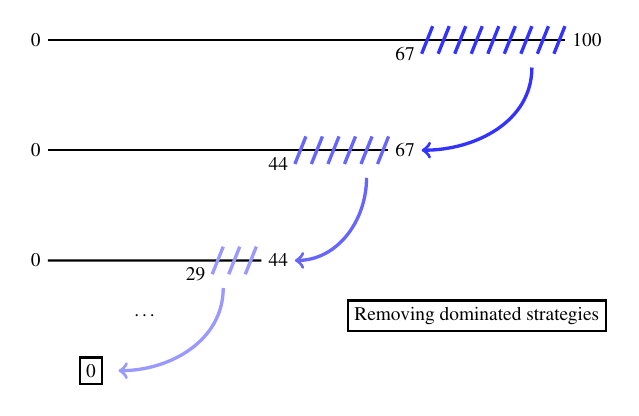
\begin{tikzpicture}[thick,scale=0.7, every node/.style={scale=0.7}]
            % First level of play
            \node (0) at (0,0) {$0$};
            \node (100) at (10,0) {$100$};
            \draw [thick] (0) -- (100);
            \node [below] at (6.7,0) {$67$};

            % Getting rid of dominated strategies
            \foreach \x in {7, 7.3, 7.6, 7.9, 8.2, 8.5, 8.8, 9.1, 9.4}
            {
                \draw [blue!80, very thick] (\x,-.25) -- (\x + .2,.25);
            }
            \draw [very thick, blue!80] (9, -.5) edge[out=270,in=0,->] (7, -2);

                % Second level of play
                \node (0) at (0,-2) {$0$};
                \node (67) at (6.7,-2) {$67$};
                \draw [thick] (0) -- (67);
                \node [below] at (4.4,-2) {$44$};

                % Getting rid of dominated strategies
                \foreach \x in {4.7, 5, 5.3, 5.6, 5.9, 6.2}
                {
                    \draw [blue!60, very thick] (\x,-2.25) -- (\x + .2,-1.75);
                }
                \draw [very thick, blue!60] (6, -2.5) edge[out=270,in=0,->] (4.7, -4);

                    % Third level of play
                    \node (0) at (0,-4) {$0$};
                    \node (44) at (4.4,-4) {$44$};
                    \draw [thick] (0) -- (44);
                    \node [below] at (2.9,-4) {$29$};

                    % Getting rid of dominated strategies
                    \foreach \x in {3.2, 3.5, 3.8}
                    {
                        \draw [blue!40, very thick] (\x,-4.25) -- (\x + .2,-3.75);
                    }

                        % Final level of play
                        \node at (2, -5) {\dots};
                        \node (0) at (1,-6) [draw] {$0$};
                        \draw [very thick, blue!40] (3.4, -4.5) edge[out=270,in=0,->] (1.5, -6);

            \node at (8, -5) [draw] {Removing dominated strategies};
        \end{tikzpicture}
    \end{center}
    \caption{Equilibrium behaviour in the two thirds of the average
    game}\label{fig:rationalisation_of_two_thirds_game}
\end{figure}

The author has used this activity on a large number of occasions and at all
times collected the data. Figure \ref{fig:histogram_of_guess} shows the
distribution of the guesses (depending on the round of play):

\begin{figure}[!hbtp]
    \begin{subfigure}{.6\textwidth}
        \centering
        \includegraphics[width=\textwidth]{static/histogram_of_guesses.pdf}
        \caption{Frequency of guesses depending on the round of play.}
        \label{fig:histogram_of_guess}
    \end{subfigure}
    \begin{subfigure}{.4\textwidth}
        \centering
        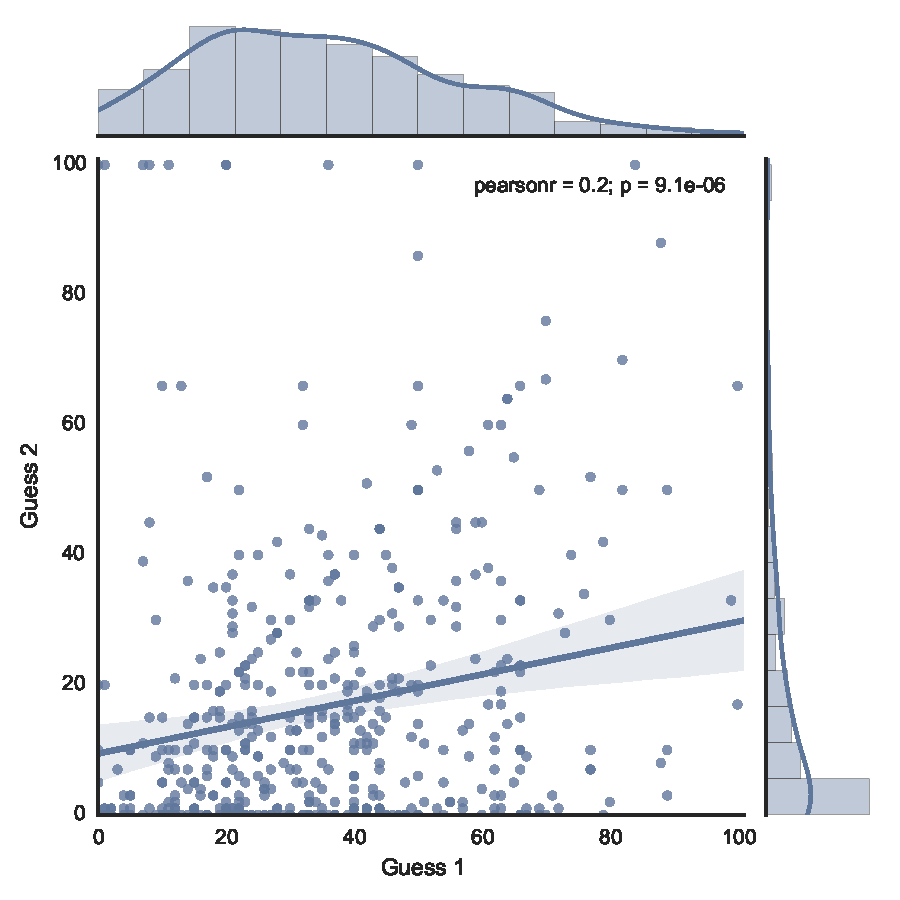
\includegraphics[width=\textwidth]{static/jointplot_of_guesses.pdf}
        \caption{Linear relationship between guesses of each round of play.}
        \label{fig:jointplot_of_guess}
    \end{subfigure}
    \caption{Results from all data collected.}
    \label{fig:all_results}
\end{figure}

We see that the second round (after the rationalisation of play described in
Figure \ref{fig:rationalisation_of_two_thirds_game}) has guesses that are closer
to the expected equilibrium behaviour.
Figure \ref{fig:jointplot_of_guess} confirms this showing the linear
relationship (albeit a weak one with \(R^2=.2\)):

\begin{equation}
    (\text{Second guess}) = .203\times(\text{First guess}) + 9.45
    \label{eq:linear_relationship}
\end{equation}

The fact that the coefficient of the relationship is less than one highlights
that the second guess is in general lower than the first guess. As can be seen
in Figure \ref{fig:all_results} not all students reduce their guess. Figure
\ref{fig:results_with_decreasing_guess} shows the results when removing these
irrational moves. In this particular case the linear relationship is in fact
stronger \(R^2=.43\):

\begin{equation}
    (\text{Second guess}) = .33\times(\text{First guess}) + 0.20
    \label{eq:linear_relationship_for_increasing_guesses}
\end{equation}

\begin{figure}[!hbtp]
    \begin{subfigure}{.6\textwidth}
        \centering
        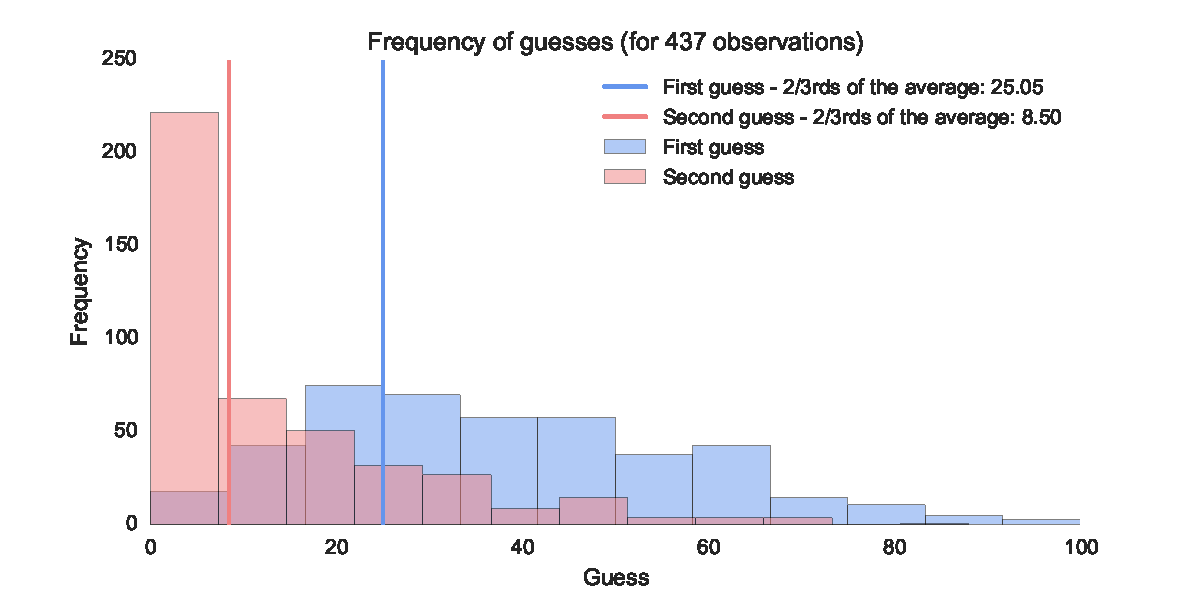
\includegraphics[width=\textwidth]{static/histogram_of_guesses_removing_increasing_guesses.pdf}
        \caption{Frequency of guesses depending on the round of play.}
        \label{fig:histogram_of_guess}
    \end{subfigure}
    \begin{subfigure}{.4\textwidth}
        \centering
        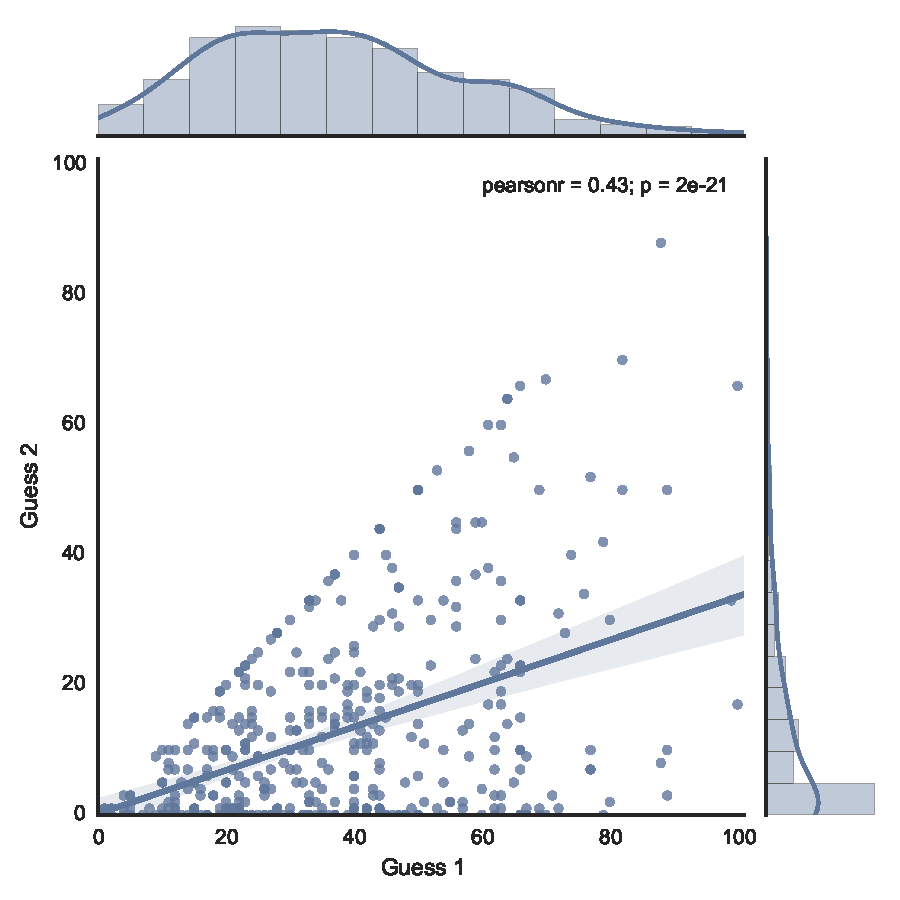
\includegraphics[width=\textwidth]{static/jointplot_of_guesses_removing_increasing_guesses.pdf}
        \caption{Linear relationship between guesses of each round of play.}
        \label{fig:jointplot_of_guess}
    \end{subfigure}
    \caption{Results from data when removing increasing guesses.}
    \label{fig:results_with_decreasing_guess}
\end{figure}

At the end of the activity, students are shown the graphical results and a
discussion had about why the theoretic equilibrium was not the winner. This
discussion usually revolves around the observation that not everyone acted
rationally and second that some participants felt like they should `spoil' the
game by guessing larger in the second round.

Finally, if time permits (and depending on the level of the participants), the
linear relationship of (\ref{eq:linear_relationship}) is used to discuss what
would happen if more rounds were to be played. In particular it is possible to
discuss ideas of convergence when generalising (\ref{eq:linear_relationship}) to
be:

\begin{equation}
    \text{Guess}_{n+1} = .203\times\text{Guess}_n + 9.45
    \label{eq:extrapolated_linear_relationship}
\end{equation}

To summarise this activity:

\begin{enumerate}
    \item Participants are explained the rules and play one round of the two
        thirds of the average game.
    \item A rationalisation and explanation of equilibrium behaviour is
        described.
    \item Participants play another round.
    \item Results are analysed and discussed.
\end{enumerate}

This activity is still quite passive in terms of physical activity (participants are
seated throughout). Nevertheless it allows the data used for the discussion of
the theory to come directly from the participants and further more all students
are active participants and there are no difficulties with regards to
encouraging participation (references to these are discussed in \cite{Rocca2010}).

\subsection{Repeated and random games}\label{sec:repeated_games}

This activity is used to introduce students to the concepts of repeated games
\cite{Maschler2013}. The mathematical details can be omitted from the initial
description of the activity to the participants but for completeness it they are
included here:

A repeated game is played over discrete time periods. Each time period is
indexed by \(0<t\leq T\) where \(T\) is the total number of periods.  In each
period \(N\) players play a static game referred to as the \textbf{stage game}
independently and simultaneously selecting actions.  Players make decisions in
full knowledge of the \textbf{history} of the game played so far (ie the actions
chosen by each player in each previous time period).  The payoff is defined
as the sum of the utilities in each stage game for every time period.

One of the most renowned repeated games is referred to as \textbf{Axelrod's
tournament} which is what is recreated in this activity \cite{Axelrod1980a,
Axelrod1980b}.

Initially a description of the prisoner's dilemma \cite{Maschler2013} is given.
The prisoner's dilemma is a simple two player game that is often used to
introduce the very basic notions of game theory. It is described by the
following two matrices:

\[
    A =
    \begin{pmatrix}
        3&5\\
        0&1
    \end{pmatrix}
    \qquad
    B =
    \begin{pmatrix}
        3&0\\
        5&1
    \end{pmatrix}
\]

The row player has utility given by \(A\) and the column player has utilities
given by \(B\).
The strategies available to each player are to cooperate: \(C\) or to defect:
\(D\). Playing \(C\) corresponds to players choosing their first row/column and
\(D\), the second row/column.

Thus if both players cooperate they both receive a utility of 3, if one player
defects, the defector gets a utility of 5 and the cooperator a utility of 0.
Finally if both players defect they receive a utility of 1. As players (in this
framework) aim to maximise their score, the Nash equilibrium for this game is
for both players to defect.

After describing this activity and in particular explaining the simple
mathematical idea of \textbf{dominated strategy} (which is what is used in the
activity of Section \ref{sec:best_responses}) participants are made aware of the
concept of Nash equilibrium. This in turn can lead to a brief description of the
tragic yet brilliant life of John Nash.

At this point the activity is described:

\begin{enumerate}
    \item All participants will form four groups/teams;
    \item Teams will \textit{duel} each other in repetitions of 5 to 8 rounds
        (depending on available time).
    \item All teams will play in a round robin tournament with cumulative scores
        being recorded.
    \item The victorious team will be the team with the highest total score.
\end{enumerate}

The tournament is run with all participants present (even those not watching).
All participants are invited to stand and confer in their teams. The importance
of standing (as a physical activity) is noted in \cite{Donnelly2011} (whilst
that reference is mainly concerned with the impact of activity on physical well
being it also describes advantages in terms of concentration).  Before every
round of every duel opposing teams are encouraged to discuss strategies, after
which they do not face each other and following a prompt hold up a card
indicating either \(C\) or \(D\).  Duels are recorded on the white board in a
table similar to the one shown in Table \ref{tab:duel}, in which two strategies
constantly cooperate (thus obtaining a utility of 3 in each round). Table
\ref{tab:duel_1} shows an example where a strategy that is alternating plays
against a strategy that always defects.

\begin{table}[!htbp]
    \caption{Playing Tit For Tat against Cooperator}
    \centering
    \begin{tabular}{ccccc}
        \toprule
        3&6&9&12&15\\
        \midrule
        3&6&9&12&15\\
        \bottomrule
    \end{tabular}
    \label{tab:duel}
\end{table}

\begin{table}[!htbp]
    \caption{Playing Alternator against Defector}
    \centering
    \begin{tabular}{ccccc}
        \toprule
        5&6&11&12&17\\
        \midrule
        0&1&1&2&2\\
        \bottomrule
    \end{tabular}
    \label{tab:duel_1}
\end{table}

Figure \ref{fig:white_board} shows a photo of a final board for a particular
implementation of this activity.

\begin{figure}[!hbtp]
    \centering
    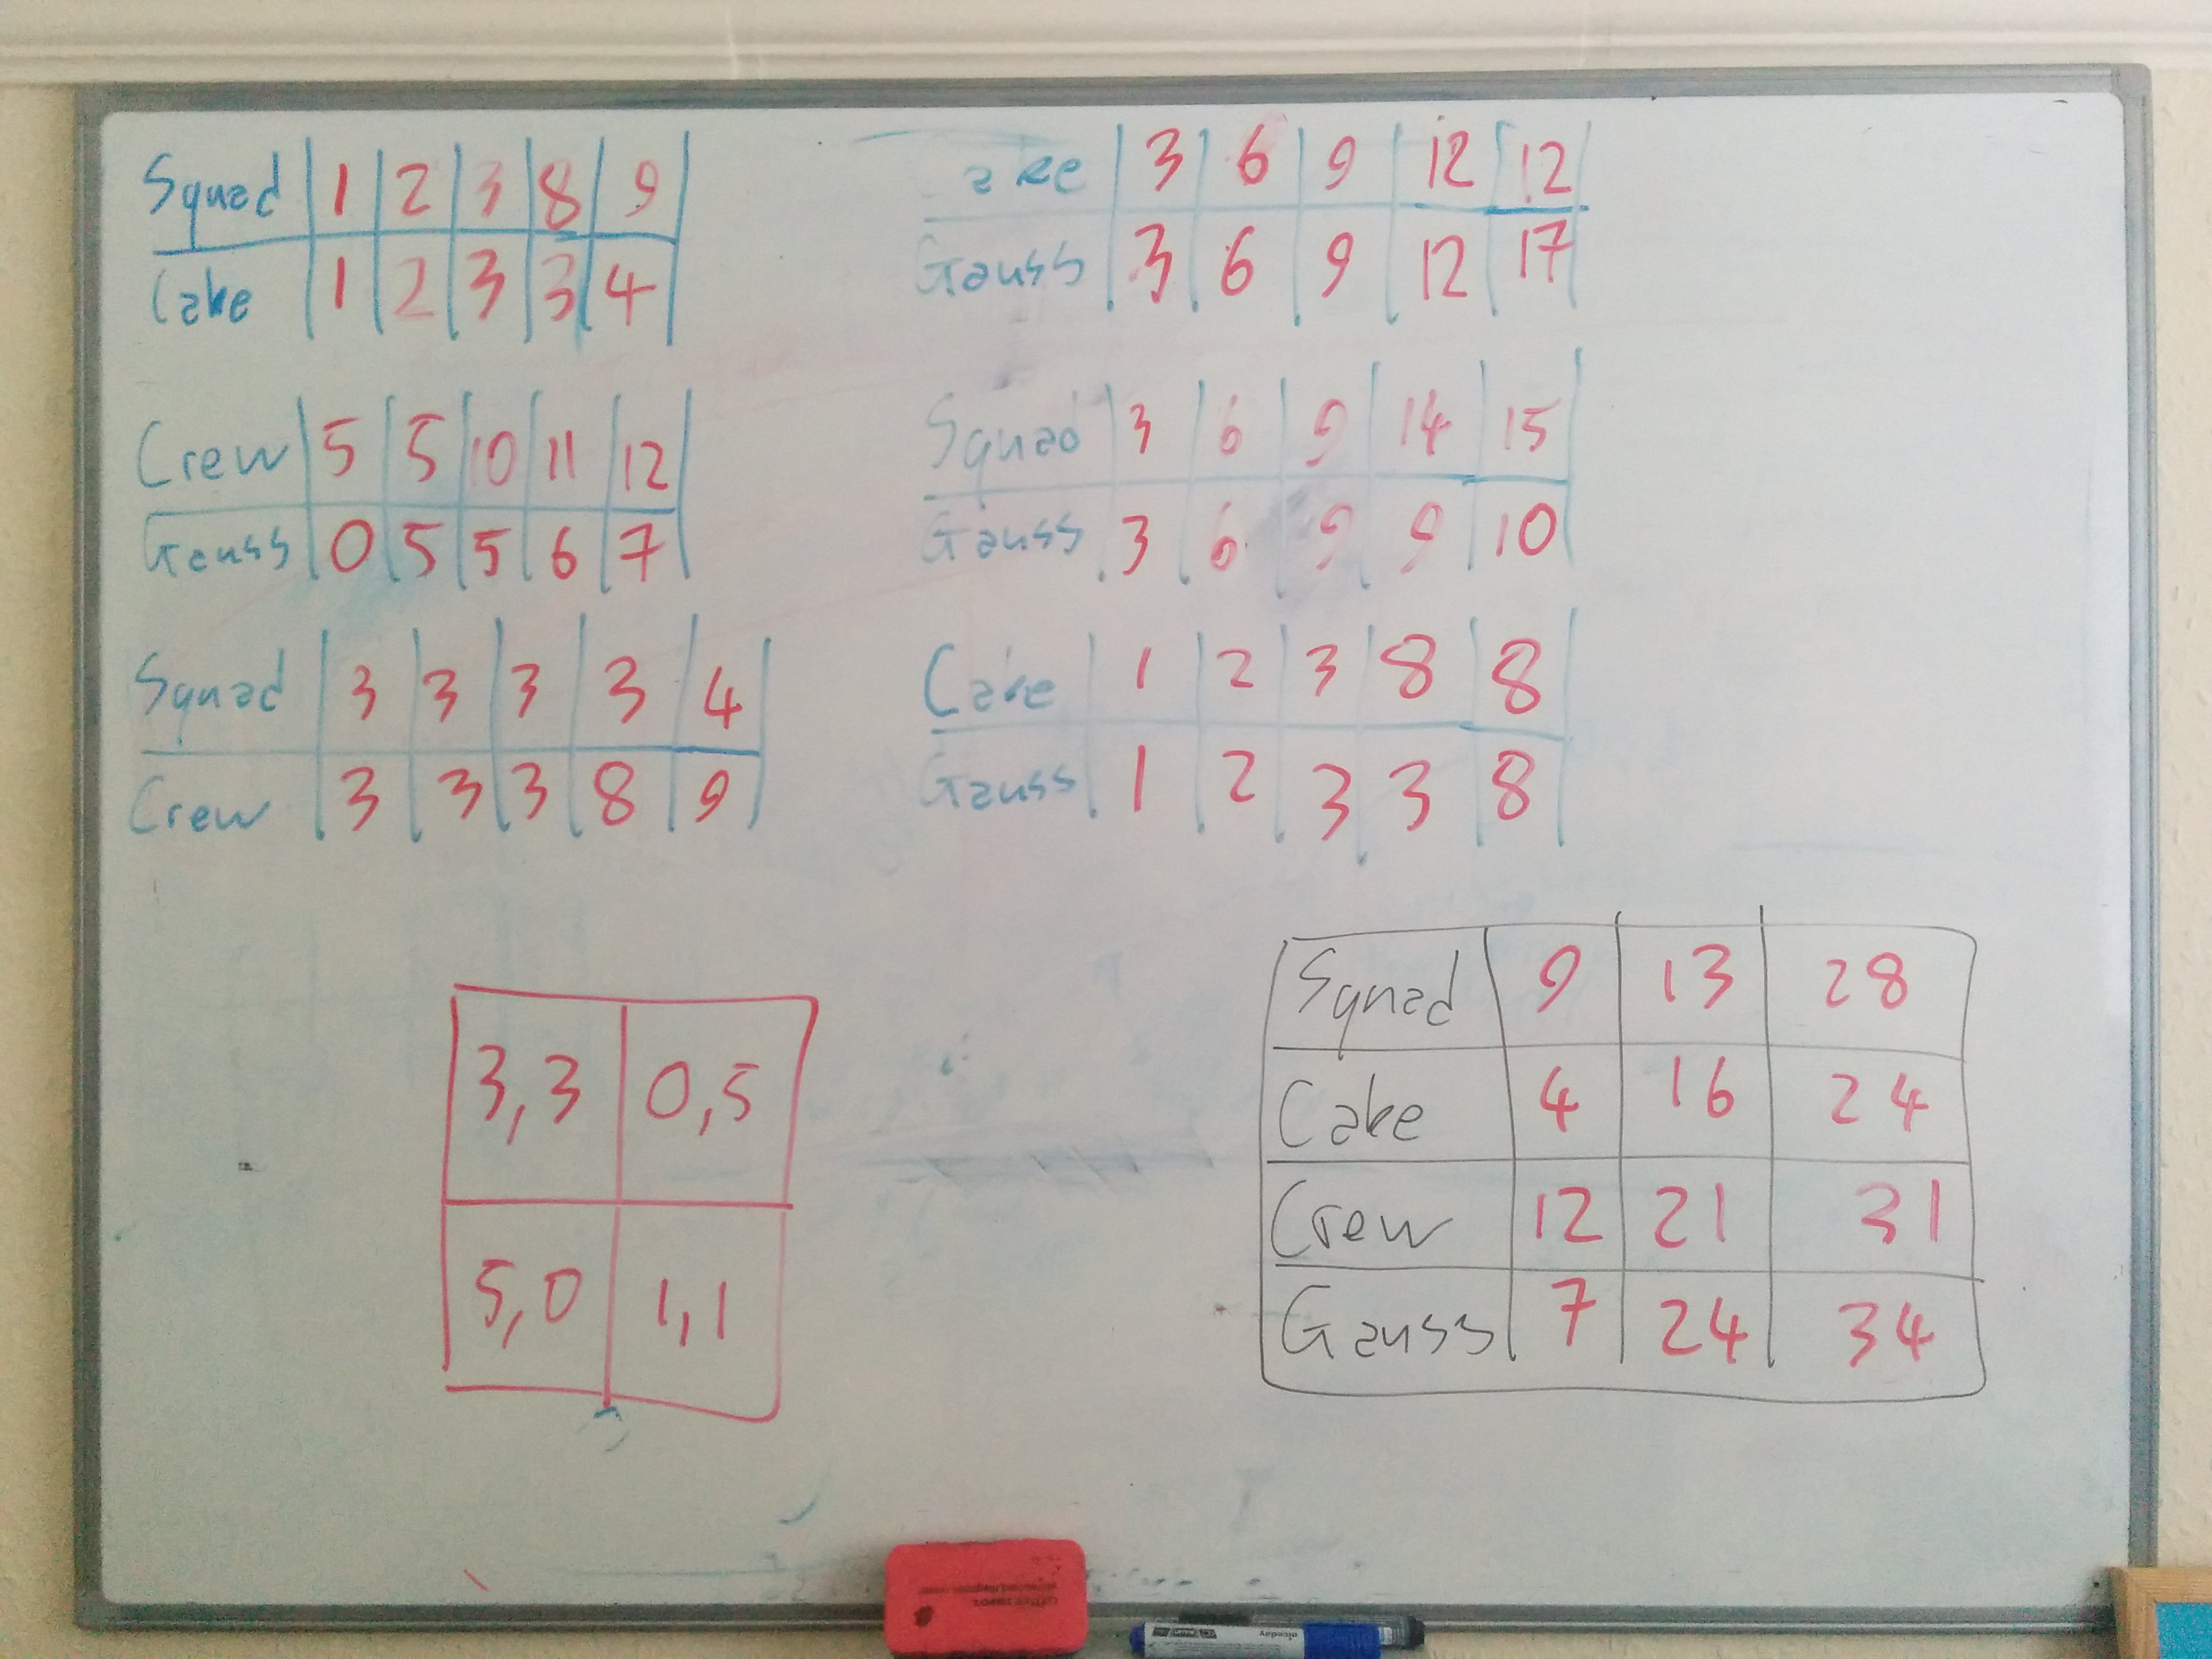
\includegraphics[width=.5\textwidth]{static/white_board.jpg}
    \caption{A photo of an actual implementation of the tournament.}
    \label{fig:white_board}
\end{figure}

The names of the strategies shown in Tables \ref{tab:duel} and \ref{tab:duel_1}
are strategies that were used in the original tournaments run by Axelrod
\cite{Axelrod1980a, Axelrod1980b}. The interesting fact of repeated games and
one that becomes apparent to participants through the activity is that whilst
repeating the stage Nash equilibrium (always defect) is indeed a Nash
equilibrium for the repeated games, this equilibrium is not unique as
reputation now has a part to play.

Note that if students do not realise this it is important to remind them that
the goal is not to win each duel but to obtain a high score. Often during the
tournament one team will (during the pre round discussion) exclaim:

\begin{quote}
   ``We will cooperate until you defect, at which point we will defect
throughout''
\end{quote}

Without realising it the participants have described a well known strategy
(\textbf{Grudger}) which takes in to account the entire history of play.

This activity can be complemented with a demonstration of software that allows
for the rapid simulation of Axelrod's tournament
\cite{Axelrod-Pythonprojectteam2015}. Figure \ref{fig:evolutionary_axelrod}
shows the performance of the strategies when put in an evolutionary context.

\begin{figure}[!hbtp]
    \centering
    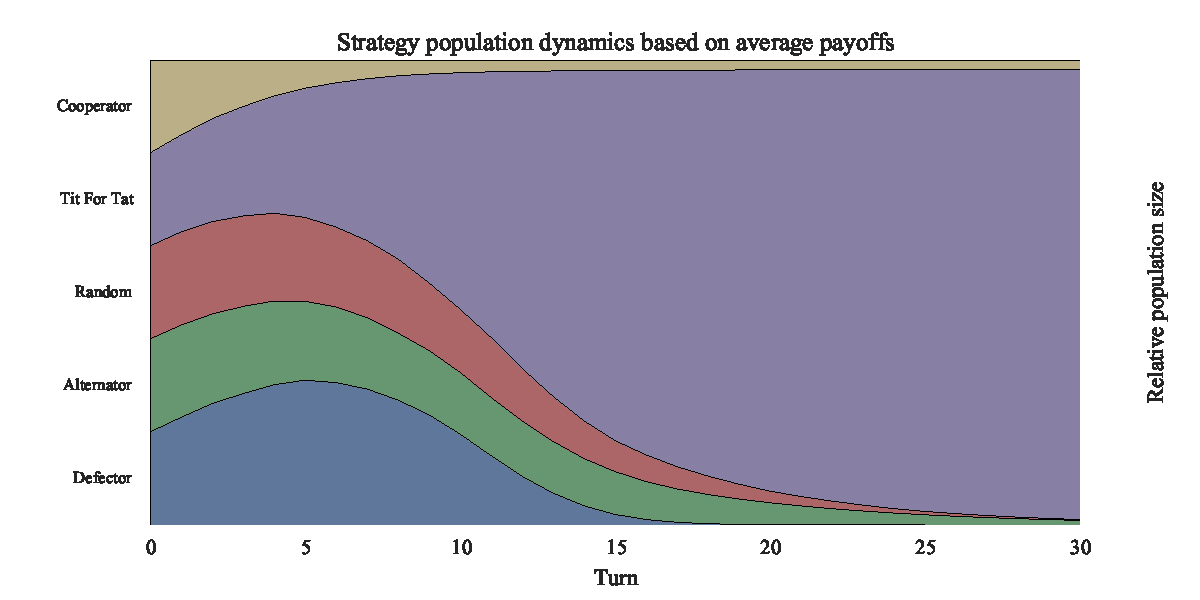
\includegraphics[width=.6\textwidth]{static/basic_strategies-reproduce.pdf}
    \caption{Repeated games in an evolutionary context.}
    \label{fig:evolutionary_axelrod}
\end{figure}

One of the inconsistencies of this approach is that all participants observe the
play by all the teams. Whilst from a mathematical perspective reputation is
inferred to mean the reputation gained during a particular duel, this has the
effect of teams being able to observe how other teams seem to play. A true
replication of Axelrod's tournament would not allow for this. One possibility
would invite participants to leave the room which might be logistically
constrained. From a pedagogic point of view however, having participants observe
the duels often leads to a much more engaged discussion (after as well as during
the activity).

This activity is usually very enjoyable and leads to a lively discussion.
Further to the fun had by participants, the theoretic discussion about repeated
games can be placed in the exact context of the tournament that was just played.

This activity can be used to introduce further game theoretic topics with
slight modifications:

\begin{itemize}
    \item \textbf{Infinitely repeated games with discounting}: the discount
        factor can be interpreted as a probability of the duel continuing for
        another round (this can be randomly sampled).
    \item \textbf{Markov games}: the two random game states can be a true game
        and an absorbing game so that this corresponds to an infinite game with
        discounting.
    \item \textbf{Evolutionary games}: the two random game states can be a true game
        and an absorbing game so that this corresponds to an infinite game with
        discounting.
\end{itemize}

\section{Summary and place within a pedagogic framework}\label{sec:summary}

These activities have been used by the author during outreach events during
which students take part in the activity of Section \ref{sec:best_responses} and
whilst the results of that are being analysed take part in the activity of
Section \ref{sec:repeated_games}. These two activities complement themselves and
form an accessible introduction to novel mathematical topics for a wide range of
age groups.

More notably however these activities have been used as part of a family of
activities used in a final year undergraduate course. This particular course is
taught in active learning pedagogic framework akin to a flipped class where
students are introduced to theoretic concepts through prior `playing of games'.
Other examples of these activities include:

\begin{itemize}
    \item \textbf{A rock paper scissors lizard tournament}: this serves as an
        introduction to mixed strategies.
    \item \textbf{A variety of games using coin flips}: this serves as an
        introduction to game with incomplete information.
    \item \textbf{Playing paper bin basketball in teams}: this serves as an
        introduction to cooperative game theory.
\end{itemize}

The general pedagogical basis for this is discussed in Section
\ref{sec:introduction} and the particular framework is shown in Figure
\ref{fig:use_of_data}. Students are active participants in the creation of
`data' which drives a discussion:

\begin{itemize}
    \item Why did you all guess this?
    \item Why did that team say that on that particular occasion?
    \item What would be a fair way of sharing the spoils for this particular
        game?
\end{itemize}

Following that discussion the theory can be put in context by highlighting
particular theoretic results and how they correspond (or not) to the behaviour
exhibited during the activity. Furthermore, this encourages an immediate
feedback with regards to student comprehension which can be reactively
addressed.

\begin{figure}[!hbtp]
    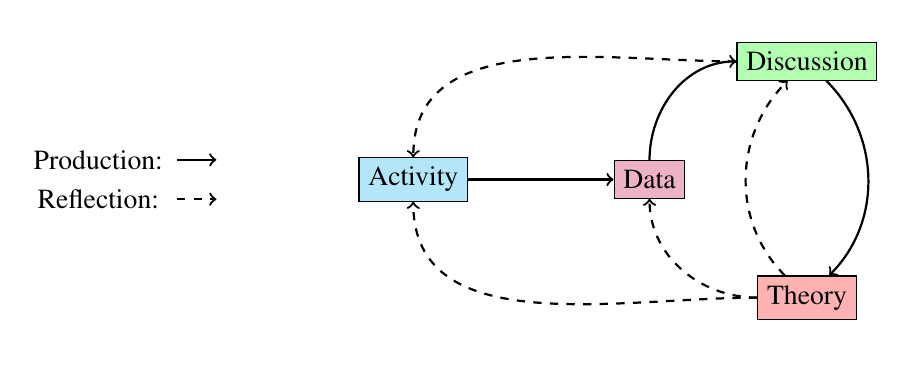
\begin{tikzpicture}
        % Nodes
        \node (activity) at (0,0) [fill=cyan!30, draw] {Activity};
        \node (data) at ($(activity) + (3,0)$) [fill=purple!30, draw] {Data};
        \node (discussion) at ($(data) + (2,1.5)$) [fill=green!30, draw] {Discussion};
        \node (theory) at ($(data) + (2,-1.5)$) [fill=red!30, draw] {Theory};

        % Creative arrows
        \draw [thick, ->] (activity) -- (data);
        \draw [thick, ->] (data) edge[out=90, in=180] (discussion);
        \draw [thick, ->] (discussion) edge[out=-45, in=45] (theory);

        % Reflective arrows
        \draw [thick, ->, dashed] (theory) edge[out=180, in=-90] (data);
        \draw [thick, ->, dashed] (theory) edge[out=180, in=-90] (activity);
        \draw [thick, ->, dashed] (discussion) edge[out=180, in=90] (activity);
        \draw [thick, ->, dashed] (theory) edge[out=135, in=-135] (discussion);

        % Key
        \draw [thick, ->] ($(activity) + (-3,.25)$) -- ($(activity) + (-2.5,.25)$);
        \node at ($(activity) + (-4, .25)$) {Production:};
        \draw [thick, ->, dashed] ($(activity) + (-3,-.25)$) -- ($(activity) +
        (-2.5,-.25)$);
        \node at ($(activity) + (-4, -.25)$) {Reflection:};

    \end{tikzpicture}
    \centering
    \caption{The active generation of data by students}
    \label{fig:use_of_data}
\end{figure}

This pedagogic approach is used throughout the course (from the first lesson)
and so after a few class meetings students are used to the high level of
participation. Here are some examples of written feedback concerning the
activities used in class:

\begin{itemize}
    \item ``Classes were fun.''
    \item ``The games helped make the content interesting.''
    \item ``This course teaches me to not trust my classmates.''
\end{itemize}

Nonetheless at the start of the course certain class management
techniques described in \cite{Rocca2010} are used. For example, the extension of
the `waiting time' for responses to questions. For students to be active
participants it is vital that they are given the time to do so.


The activities described in Section \ref{sec:game_theory} are particular to game
theory however the author does not feel that the general pedagogic strategy
outlined in Figure \ref{fig:use_of_data} is constrained to a particular course.
Similar activities could be devised in other subjects where students generate
`data' than aids the contextualisation of theory so as to aspire to not only a
constructive learning model but also a social one.

\printbibliography
\end{document}
